\section*{Introduction}\label{sec:introduction} % (fold)
This report explores the implementation and analysis of a 2D Lennard-Jones molecular dynamics simulation. In this project, we focus on two fundamental ensemble types in molecular mechanics: the microcanonical ensemble (NVE) and the canonical ensemble (NVT). \\
\\
The microcanonical ensemble (NVE) simulates an isolated system with a constant number of particles (N), volume (V), and total energy (E). The canonical ensemble (NVT), on the other hand, also has a constant number of particles (N) and volume (V), but in this case we keep the temperature (T) constant instead of the energy. This is done, in our case, by using a Berendsen thermostat.\\
\\
Both types of simulations employ the truncated Lennard-Jones potential, which models both the attractive and repulsive forces between particles.
\begin{equation}
	U_{\text {trunc }}(r)=\left\{\begin{array}{l}
		U(r)-U\left(r_c\right), \quad r \leq r_c \\ 0, \quad r>r_c \end{array} \quad, \text { with } \quad U(r)=4\left[\left(\frac{1}{r}\right)^{12}-\left(\frac{1}{r}\right)^6\right]\right.
\end{equation}
This potential is a fundamental model in computational physics and is most often used to accurately represents the behavior of noble gases. Furthermore the velocity-Verlet integration scheme is used to solve the equations of motion with the promise of having good computational efficiency and numerical stability.\\
\\
To improve performance, a cell lists based approach for finding neighboring particles, with the goal of significantly reducing the computational complexity from $O(N^2)$ to $O(N)$. In order to enhance our understand of the system, several key properties of the sytem were analyzed. This includes energy conservation, temperature equilibration, and the radial distribution, providing key insights into the structural organization of particles. \\
\\
By examining different temperatures and particle counts this project explores how system size and thermal energy affect particle dynamics and structural properties in both NVE and NVT ensembles.\\
\\
This project was implement using Python, for further information regarding the implementation, consult the README provided in projects root folder.

% section Introduction (end)
\section{Energy-Conserving Dynamics: The NVE Ensemble}\label{sec:energy_conserving_dynamics_the_nve_ensemble} % (fold)
% The microcanonical ensemble (NVE) represents an isolated system with fixed number of particles (N), volume (V), and total energy (E). In an ideal NVE simulation, the total energy should remain constant, providing a critical validation metric for our implementation. 
For the NVE simulation several different starting configurations were explored. The figure shown in the report were down with 100, 400 and 900 particles and varying timesteps, namely 0.01, 0.02 and 0.005 in order to evaluate the systems energy conservation properties and equilibration.
\subsection{Energy Conservation}
In Figure~\ref{fig:energy_conservation} one can observe the evolution of the kinetic, potential and total energy. All simulations show the expected behavior of constant total energy, while kinetic and potential energies evolve in a complementary pattern, which represent the constant exchange between the two types of energy. Please note that the equilibration period is included in these graphs, which allows us to analyze the time needed for the system to get to a equilibrium state.\\
\\
For a system with fewer particle, the graphs are showing that relative fluctuations in both kinetic and potential are larger in comparison to system with more particles. This behavior is expected, then large system usually show a more stable properties, due to the law of large numbers. Furthermore the time required to reach an equilibrium also takes longer in for smaller system in comparison to larger systems. 
\begin{figure}[H]
	\centering
	\begin{subfigure}{0.5\textwidth}
		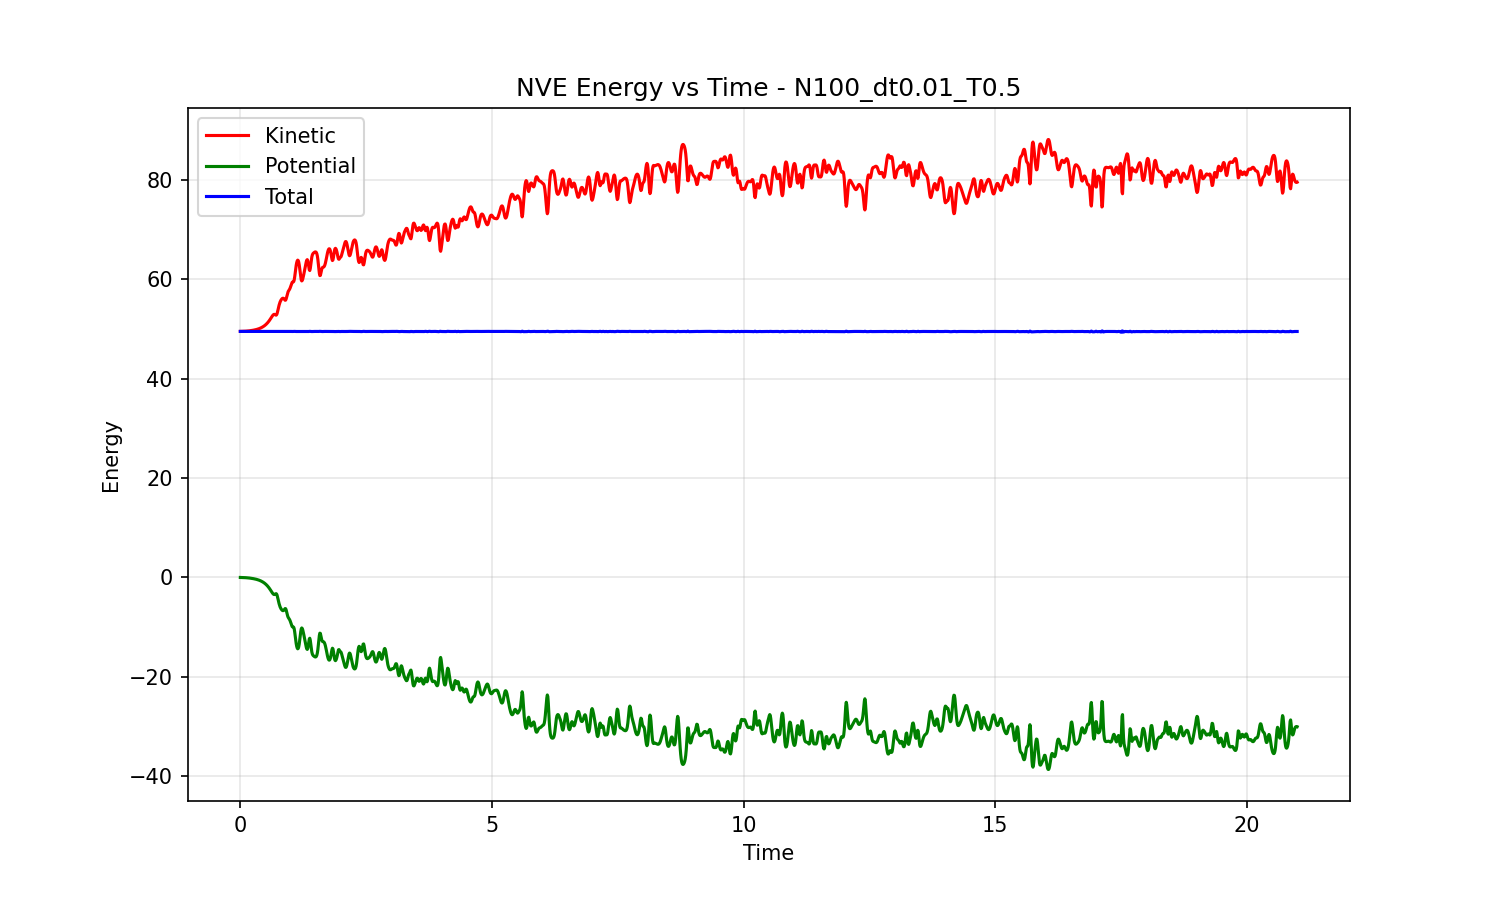
\includegraphics[width=\textwidth]{media/energy_N100_dt0.01_T0.5.png}
		\caption{N=100 particles with dt=0.01 and T=0.5}
		\label{sfig:energy_N100}
	\end{subfigure}%
	~
	\begin{subfigure}{0.5\textwidth}
		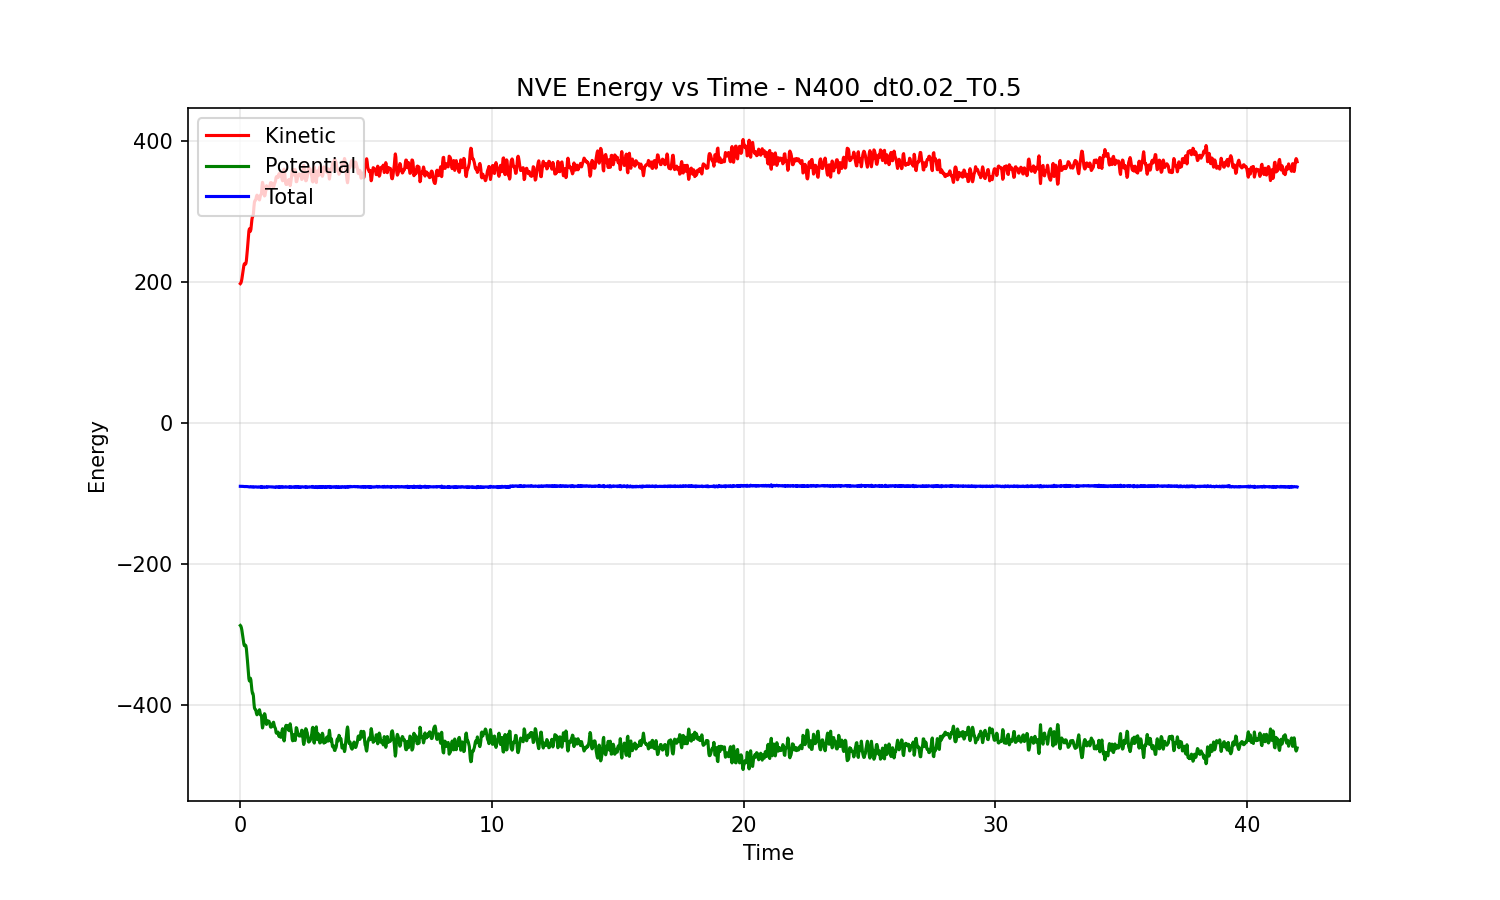
\includegraphics[width=\textwidth]{media/energy_N400_dt0.02_T0.5.png}
		\caption{N=400 particles with dt=0.02 and T=0.5}
		\label{sfig:energy_N400_dt002}
	\end{subfigure}%
	\\
	\begin{subfigure}{0.5\textwidth}
		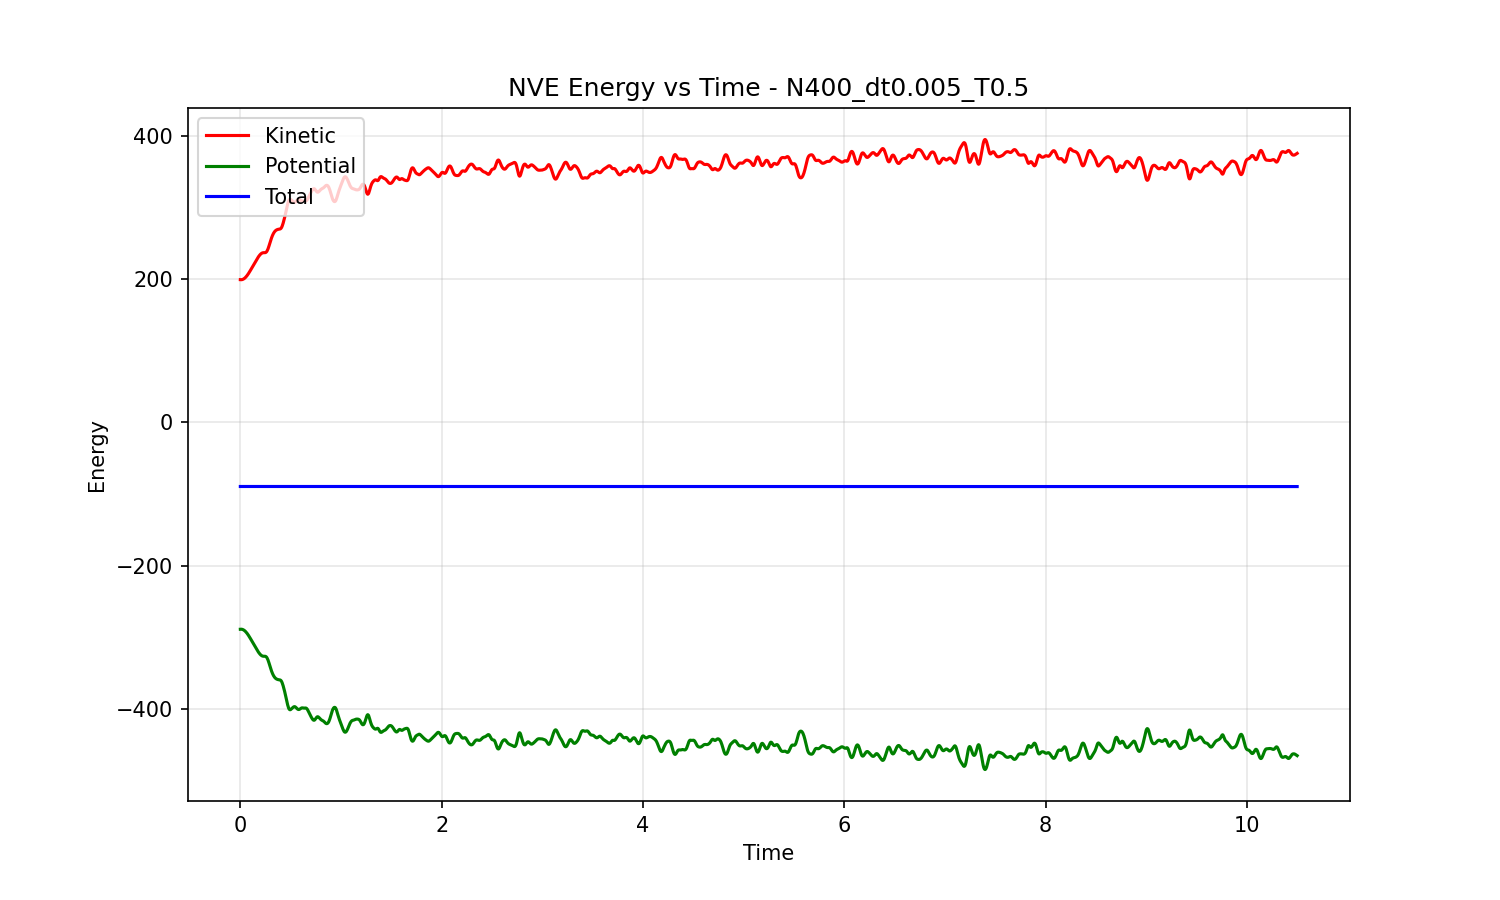
\includegraphics[width=\textwidth]{media/energy_N400_dt0.005_T0.5.png}
		\caption{N=400 particles with dt=0.005 and T=0.5}
		\label{sfig:energy_N400_dt0005}
	\end{subfigure}%
	~
	\begin{subfigure}{0.5\textwidth}
		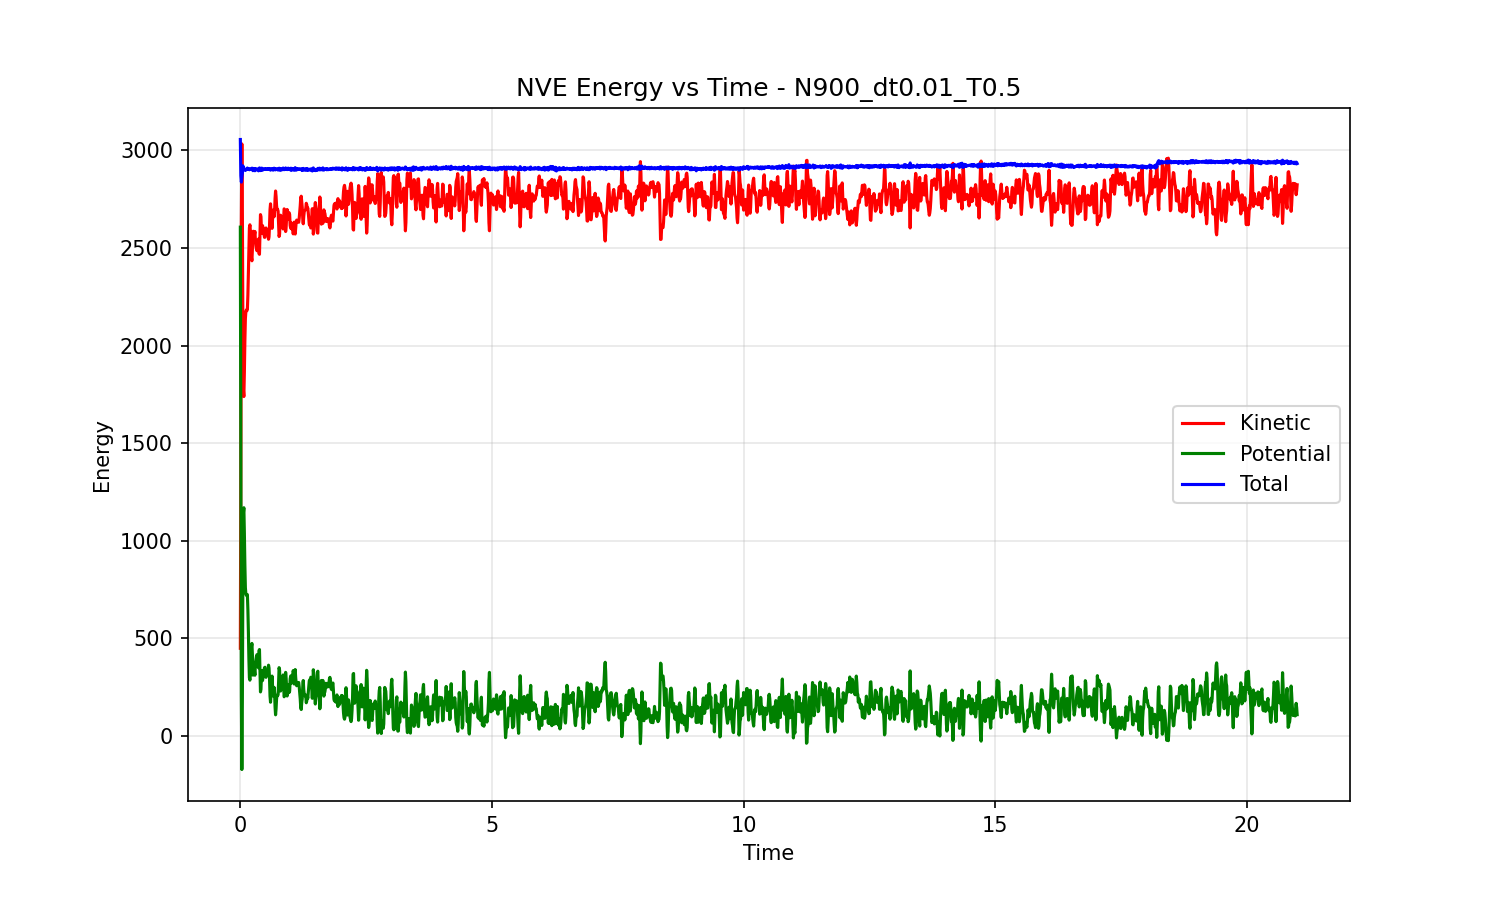
\includegraphics[width=\textwidth]{media/energy_N900_dt0.01_T0.5.png}
		\caption{N=900 particles with dt=0.01 and T=0.5}
		\label{sfig:energy_N900}
	\end{subfigure}%
	\caption{\textbf{Energy Conservation in NVE Ensemble} 
    Analysis of total, kinetic, and potential energies over time for different system configurations.}
	\label{fig:energy_conservation}
\end{figure}
\subsection{Time Step Dependence}
Figure~\ref{fig:energy_error} yields a crucial insight into the choice of a proper time step, by looking at the energy conservation error as a function of time.
When comparing two simulation with the same size (in our case $N=400$) and different time steps $dt=0.02,0.005$ we can make the following key observations, that the simulation with the large ($dt = 0.02$) step size, shows an significantly larger energy conservation error in comparison to the lower time step of $dt = 0.005$. This confirms the expected error that the velocity-Verlet integration scheme has, where for smaller time steps the scheme is more accurate resulting in a smaller energy conservation error.

\subsection{Temperature Evolution}
Figure~\ref{fig:temperature_evolution} depicts the evolution of temperature over the duration of the simulation including the "warmup" period.
We observe in all cases an initial temperature adjustment, followed by fluctuations 
around a constant temperature. Unlike the NVT ensemble where we have a target temperature, these NVE simulations have an initial temperature and then it evolves freely, based on the system dynamics. This is expected in NVE simulations due to the energy redistribution between kinetic and potential energy until the system reaches a natural equilibrium. We can observe that these fluctuations decrease when the number of particles increases and vice versa. These equilibrium times closely resemble the observed that of the energy evolution seen in Figure~\ref{fig:energy_conservation}.

\subsection{Momentum Conservation}
While not explicitly shown in the figures, all the simulation exhibit zero total momentum through out the complete simulation. In the real time visualization of this project, the indicator for total momentum is displayed. This conservation confirmed the proper implementation of the periodic boundary conditions and other physical properties.


\begin{figure}[H]
	\centering
	\begin{subfigure}{0.45\textwidth}
		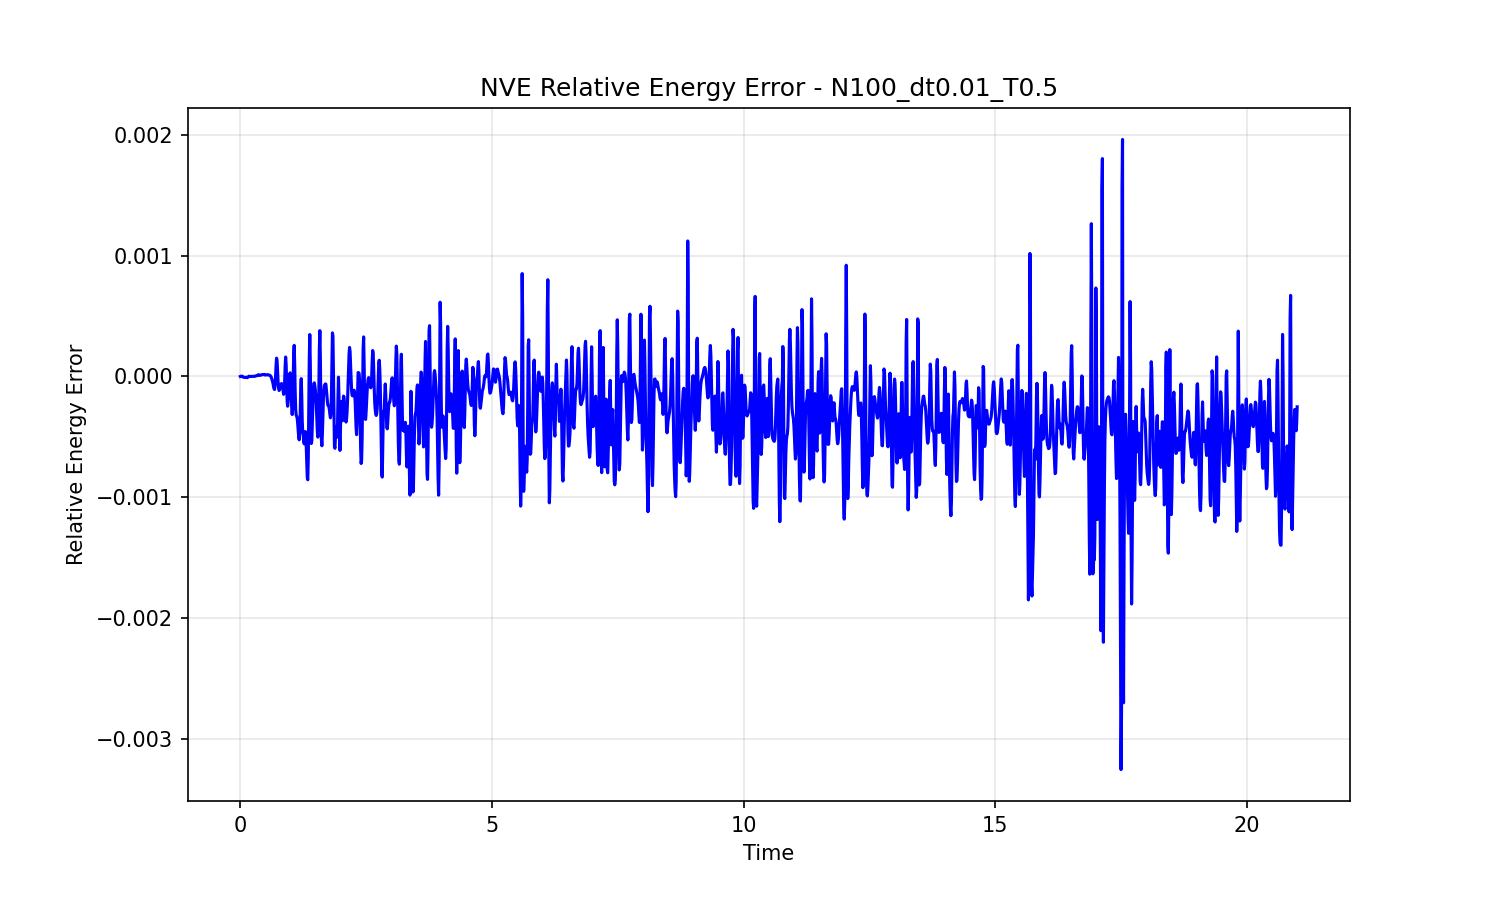
\includegraphics[width=\textwidth]{media/error_N100_dt0.01_T0.5.png}
		\caption{N=100 particles with dt=0.01 and T=0.5}
		\label{sfig:error_N100}
	\end{subfigure}%
	~
	\begin{subfigure}{0.45\textwidth}
		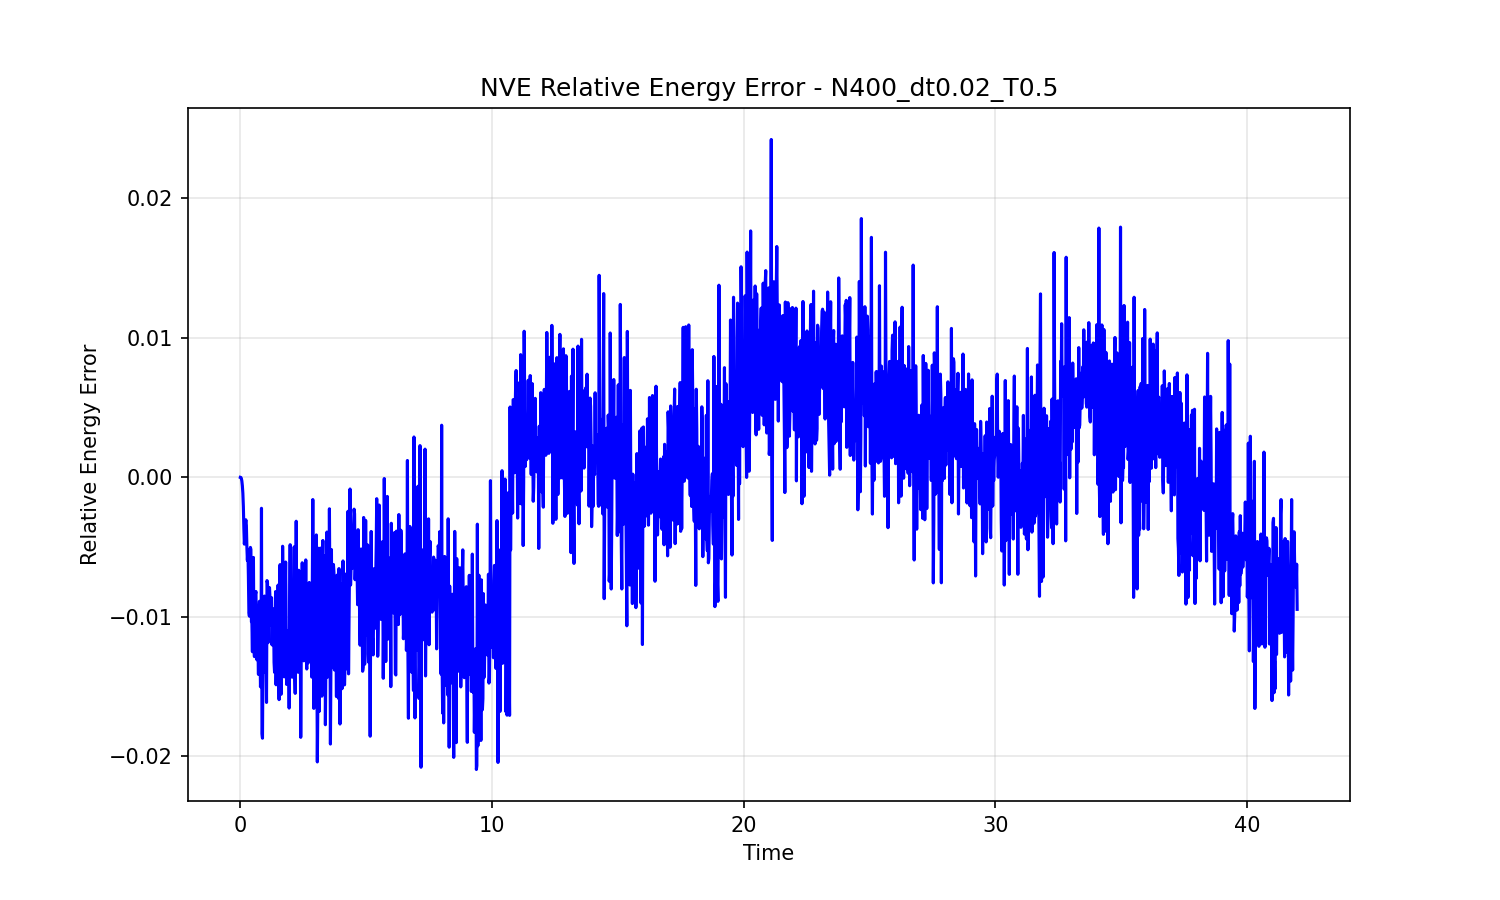
\includegraphics[width=\textwidth]{media/error_N400_dt0.02_T0.5.png}
		\caption{N=400 particles with dt=0.02 and T=0.5}
		\label{sfig:error_N400_dt002}
	\end{subfigure}%
	\\
	\begin{subfigure}{0.45\textwidth}
		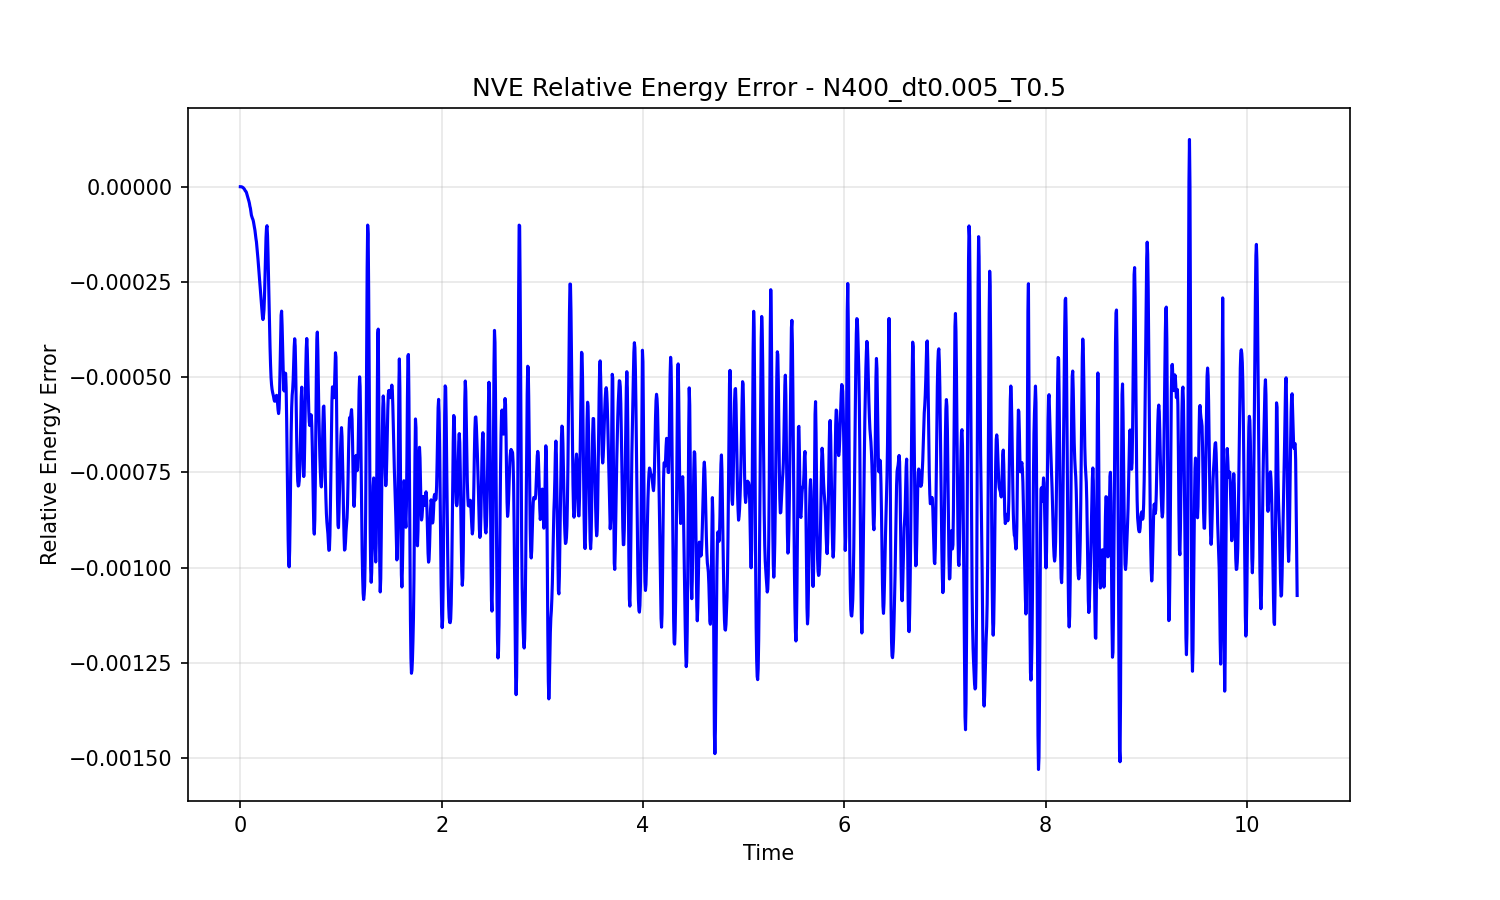
\includegraphics[width=\textwidth]{media/error_N400_dt0.005_T0.5.png}
		\caption{N=400 particles with dt=0.005 and T=0.5}
		\label{sfig:error_N400_dt0005}
	\end{subfigure}%
	~
\begin{subfigure}{0.45\textwidth}
		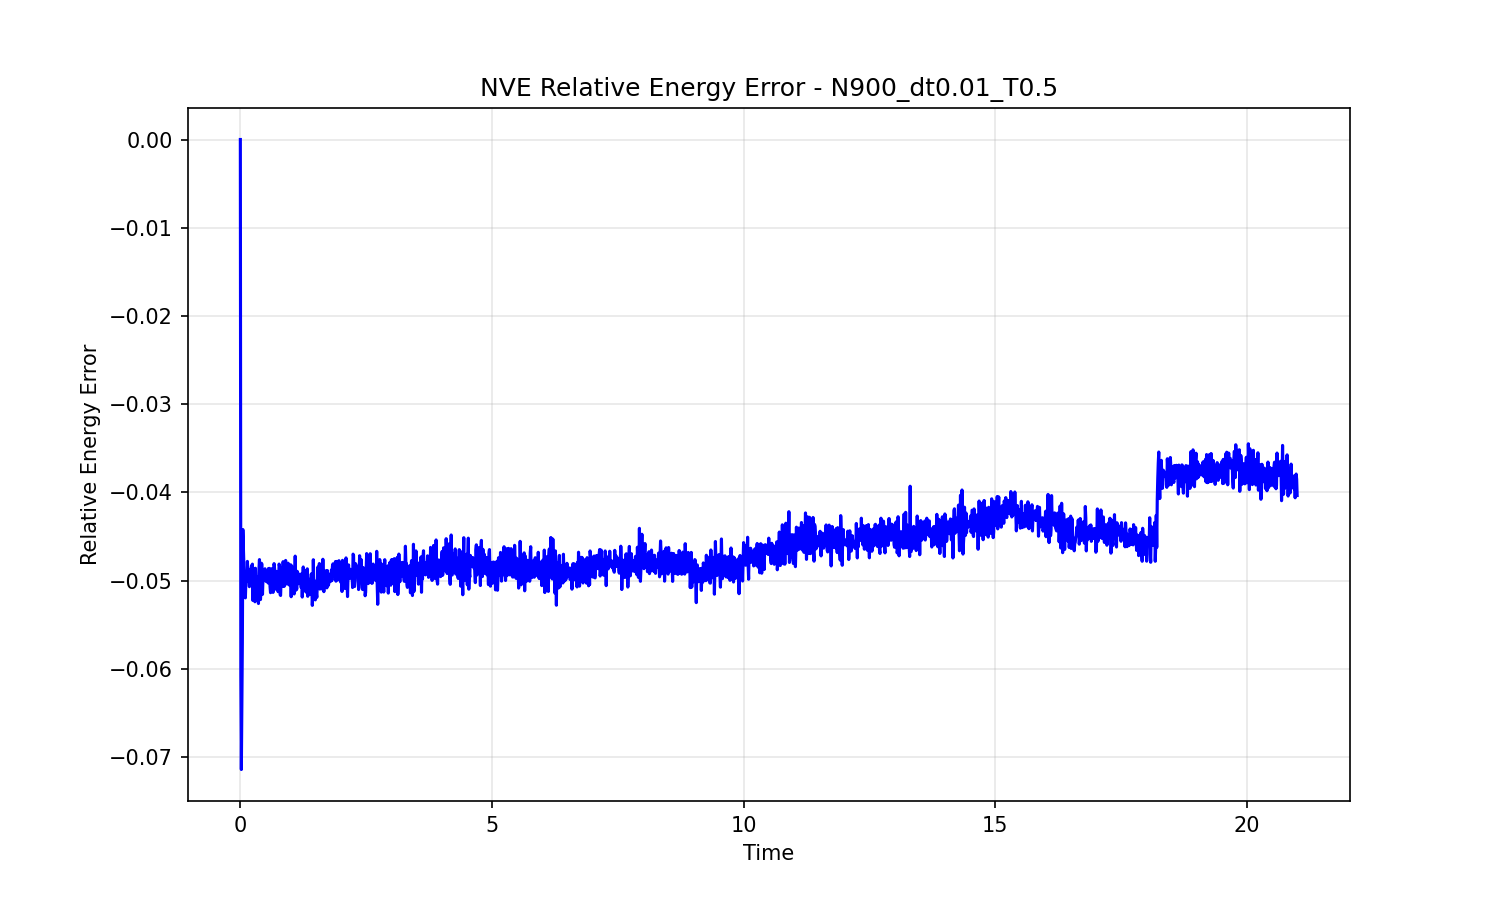
\includegraphics[width=\textwidth]{media/error_N900_dt0.01_T0.5.png}
		\caption{N=900 particles with dt=0.01 and T=0.5}
		\label{sfig:error_N900}
	\end{subfigure}%

	\caption{\textbf{Energy Conservation Error Analysis in NVE Ensemble} 
	Relative energy conservation error over time for different system configurations.}
	\label{fig:energy_error}
\end{figure}

\begin{figure}[H]
	\centering
	\begin{subfigure}{0.45\textwidth}
		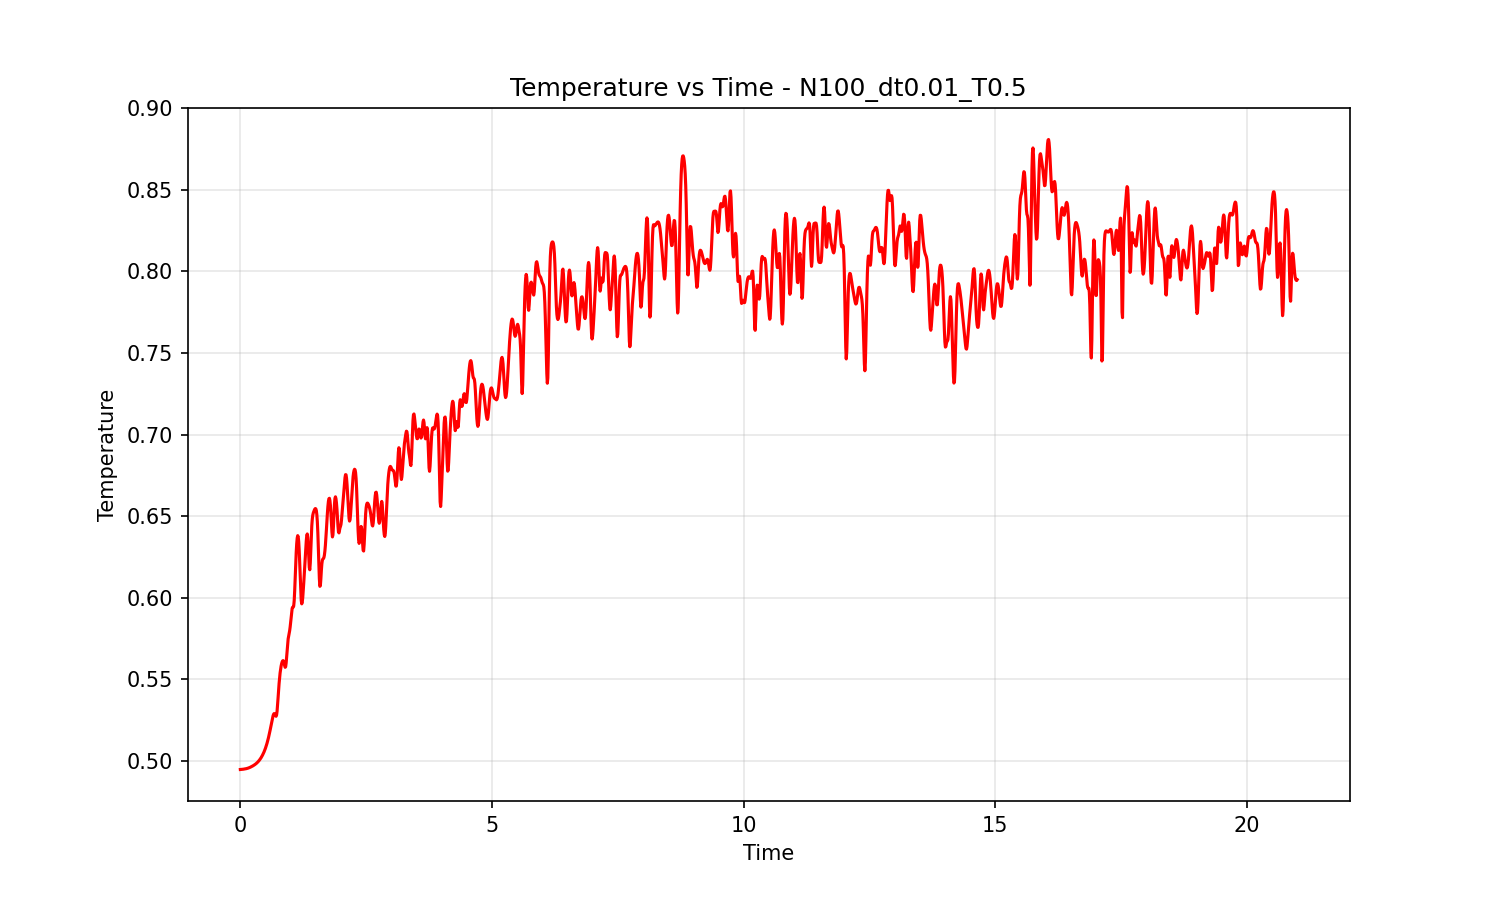
\includegraphics[width=\textwidth]{media/temp_N100_dt0.01_T0.5.png}
		\caption{N=100 particles with dt=0.01 and T=0.5}
		\label{sfig:temp_N100}
	\end{subfigure}%
	~
	\begin{subfigure}{0.45\textwidth}
		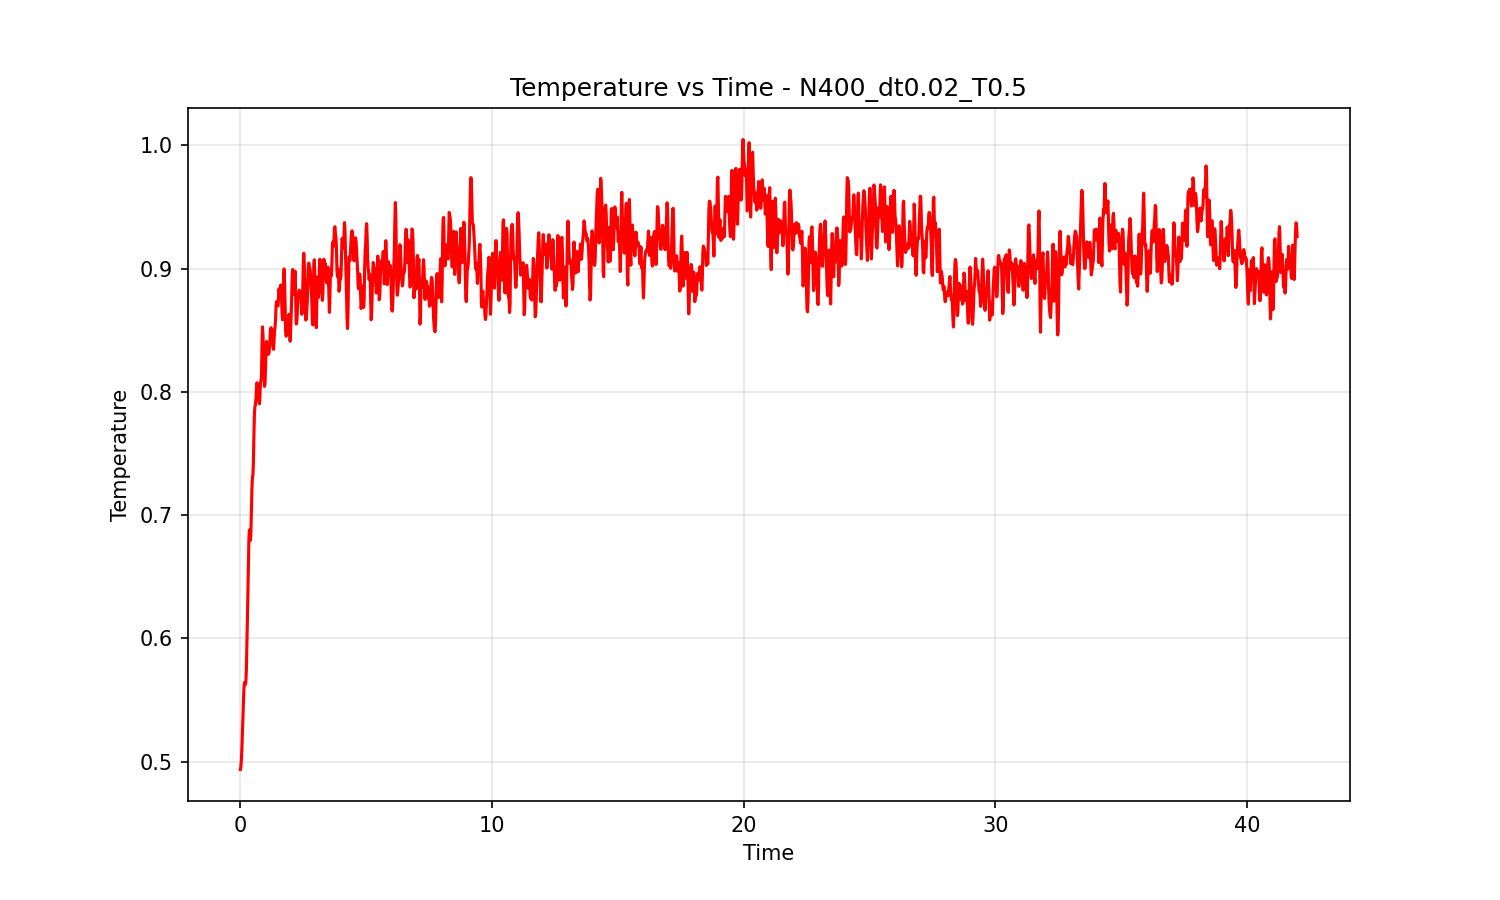
\includegraphics[width=\textwidth]{media/temp_N400_dt0.02_T0.5.png}
		\caption{N=400 particles with dt=0.02 and T=0.5}
		\label{sfig:temp_N400_dt002}
	\end{subfigure}%
	\\
	\begin{subfigure}{0.45\textwidth}
		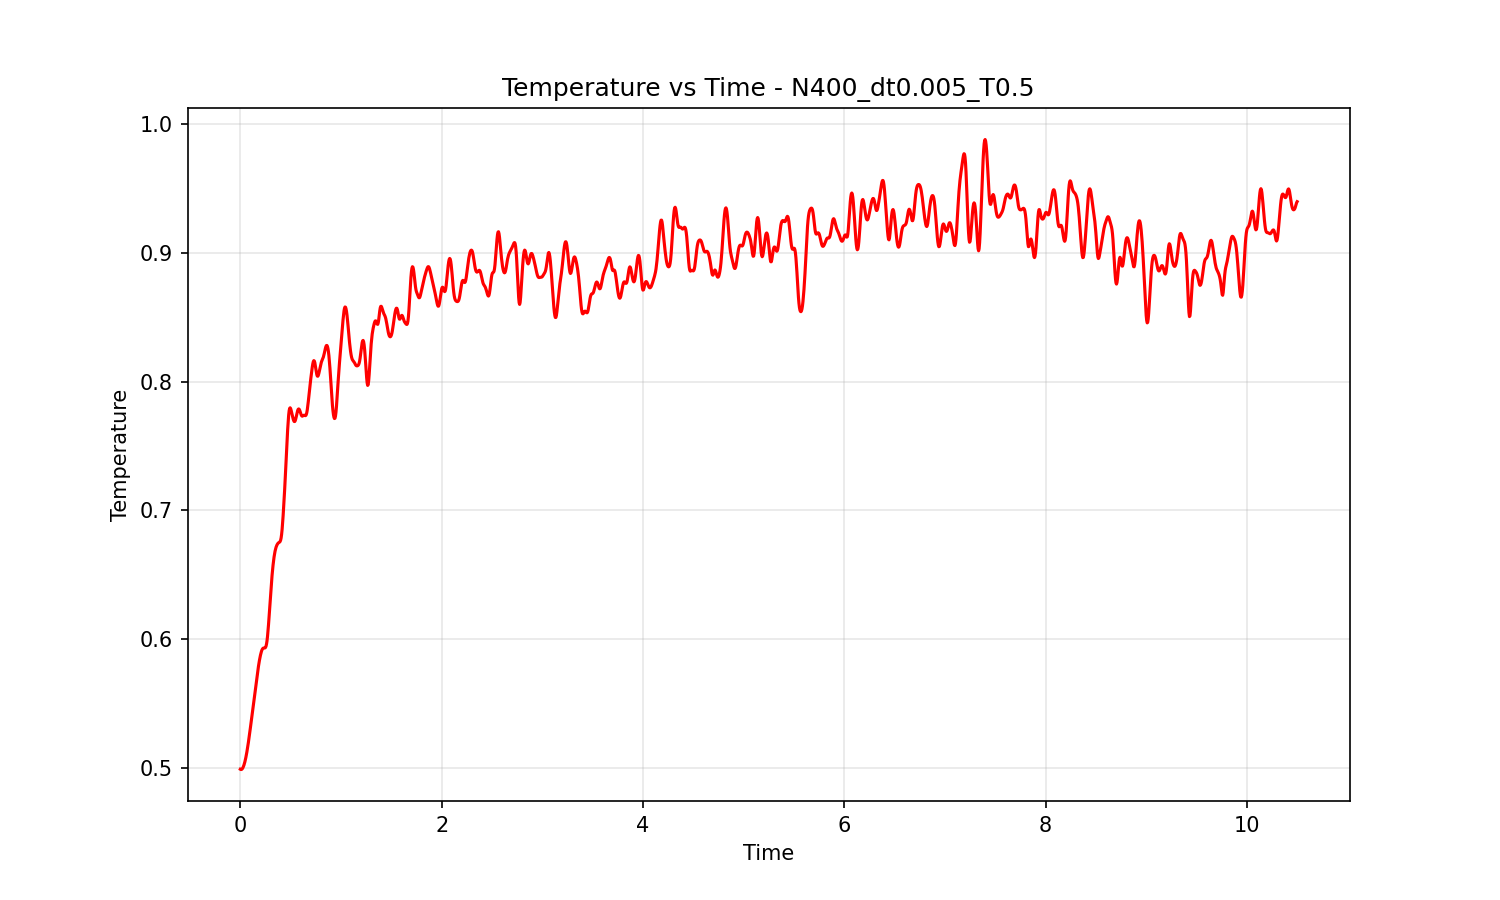
\includegraphics[width=\textwidth]{media/temp_N400_dt0.005_T0.5.png}
		\caption{N=400 particles with dt=0.005 and T=0.5}
		\label{sfig:temp_N400_dt0005}
	\end{subfigure}%
	~
	\begin{subfigure}{0.45\textwidth}
		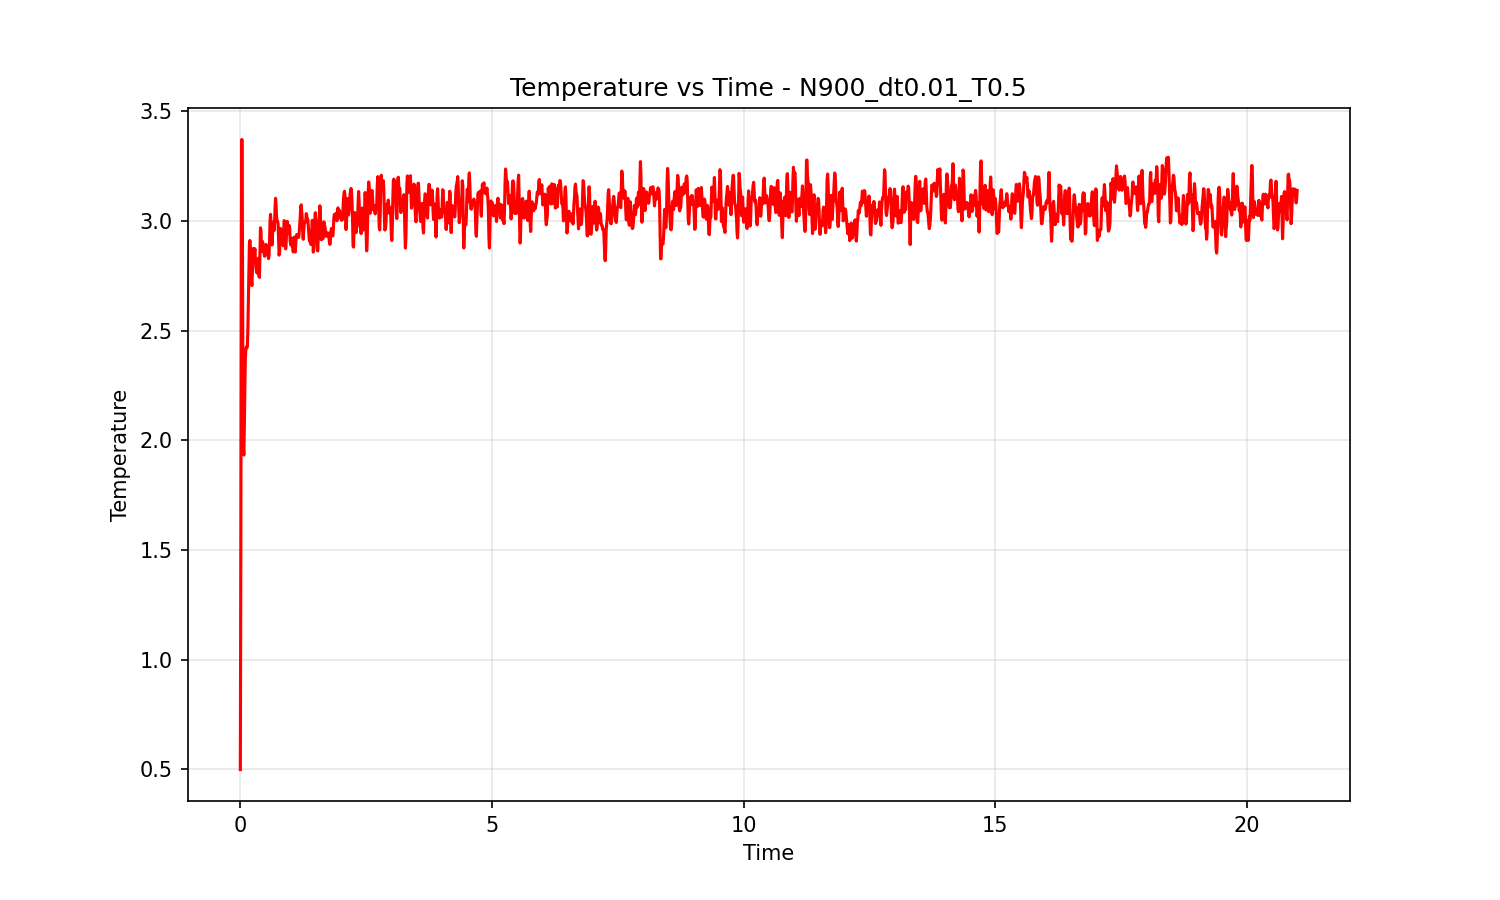
\includegraphics[width=\textwidth]{media/temp_N900_dt0.01_T0.5.png}
		\caption{N=900 particles with dt=0.01 and T=0.5}
		\label{sfig:temp_N900}
	\end{subfigure}%
	\caption{\textbf{Temperature Evolution in NVE Ensemble} 
	Analysis of temperature fluctuations over time for different system configurations.}
	\label{fig:temperature_evolution}
\end{figure}
% section Energy-Conserving Dynamics: The NVE Ensemble (end)
